\documentclass[12pt]{article}
\usepackage[utf8]{inputenc}
\usepackage[margin=1in]{geometry}
\usepackage{graphicx}
\usepackage{amsmath}
\usepackage{natbib}
\usepackage{hyperref}
\usepackage{setspace}
\usepackage{xcolor}
\usepackage{caption}
\usepackage{subcaption}
\usepackage{booktabs}
\usepackage{float}
% \usepackage{textcomp} % For micro symbol

% Fix for Unicode symbols
\DeclareUnicodeCharacter{03BC}{\ensuremath{\mu}} 

\title{\textbf{Ancient Anorthositic Complexes: Widespread in Lower Martian Crust}}
\author{Michael S. Phillips\textsuperscript{1}\\ 
Christina E. Viviano\textsuperscript{2}\\
A. Deanne Rogers\textsuperscript{3}\\
Linae Larson\textsuperscript{1}\\
Livio Tornabene\textsuperscript{4}\\
Alexander Trowbridge\textsuperscript{5}\\
Jeffrey E. Moersch\textsuperscript{6}\\
Harry Y. McSween Jr.\textsuperscript{6}}

\begin{document}

\maketitle

\begin{flushleft}
\textsuperscript{1}Lunar and Planetary Laboratory, University of Arizona, Tucson, AZ, USA.\\
\textsuperscript{2}Johns Hopkins University Applied Physics Laboratory, Laurel, MD, USA.\\
\textsuperscript{3}Department of Geosciences, Stony Brook University, Stony Brook, NY, USA.\\
\textsuperscript{4}Department of Earth and Environmental Sciences, University of Waterloo, Waterloo, ON, Canada.\\
\textsuperscript{5}Department of Earth Sciences, Western University, London, ON, Canada.\\
\textsuperscript{6}Department of Earth and Planetary Sciences, University of Tennessee, Knoxville, TN, USA.\\
\end{flushleft}

\newpage
\section*{Abstract}
\setlength{\parindent}{0em} % Set the paragraph indentation to 1em
\setlength{\parskip}{6pt}   % Remove extra spacing between paragraphs
We report extensive detections of feldspathic, possibly anorthositic, lithologies within outcrops uplifted by the Argyre basin-forming impact on Mars. The radial position of feldspathic outcrops indicates they are stratigraphically above olivine-bearing material and below low-calcium pyroxene-bearing rocks, and the inferred depths suggest that feldspathic lithologies are present in the lower martian crust in the circum-Argyre region. This stratigraphy bears striking resemblance to that observed at the Hellas basin rim and indicates that feldspathic rocks could be pervasive within the lower crust across the entire southern highlands of Mars. These results are consistent with evidence from geophysical data suggesting a lower-density lower crust, but likely not sufficient to fully explain the expected lower density. Importantly, these feldspathic rocks are present alongside pyroxene- and olivine-bearing units, a suite of compositions commonly associated with layered mafic intrusions (LMI). We suggest that a process early in Mars' history produced large volumes of melt that cooled slowly to form LMI-like complexes and that these complexes represent primary martian crust. The melt-producing process ostensibly affected the whole southern hemisphere, and possibly the globe. These observations offer direct evidence to support and refine existing models of early crust formation, addressing key questions regarding crustal density variations and formation mechanisms that have previously lacked widespread observational constraints.

\section*{Main}

In contrast to Earth and Venus, Mars preserves a surface rock record dating back to $\sim$4.55 Ga \citep{Humayun2013, Kruijer2020}. The preservation of ancient rocks ($\geq$4.1 Ga, pre-Noachian) at the surface provides a unique opportunity to study early crustal formation through remote sensing. Understanding how and when evolved rocks first formed on terrestrial planets remains a major open question in planetary geology. Since the processes that formed Mars' primary crust share more similarities with Earth- and Venus-sized bodies than with lunar-sized bodies \citep{Elkins-Tanton2012}, studying the oldest Martian crust provides critical insights into early crustal evolution across terrestrial planets.

Noteworthy among the ancient rocks of Mars are compositions apparently dominated by plagioclase feldspar (Fig.~\ref{fig:global_distribution}). Ancient feldspathic and silicic rocks provide clear evidence that crustal differentiation occurred early in Mars' history \citep[e.g.,][]{Stolper2013, Sautter2015}, although the mechanism was likely fractional crystallization of basaltic magmas rather than plate-tectonic processes that form continental crust on Earth \citep{Udry2018}. Whether such differentiation occurred only at isolated locations or globally is an open question. Here, we present evidence for a widespread, plagioclase-rich component to the lower martian crust that likely spans the entire southern highlands. Our results suggest a hemispheric, if not global, process that resulted in differentiated magmas over $\sim$4.1 billion years ago on Mars.

Though increasingly recognized as important constituents of the Martian crust, feldspathic rocks are relatively rare compared to basaltic materials based on orbital observations \citep{McSween2009, McSween2015, McSween2023}. Many detections of plagioclase-rich compositions come from isolated exposures in Noachian and older terrains in the southern highlands, interpreted as possible intrusive bodies \citep{Quantin2012, Carter2013, Wray2013, Sautter2016, Payre2022}. Other plagioclase-rich occurrences are linked to likely volcanic units found in Hesperian-aged terrains, such as Syrtis Major \citep{Eggers2021}, western Arcadia Planitia \citep{Farrand2021, Rogers2022}, and the Eridania basin \citep{Michalski2023}.

Other studies have revealed more extensive occurrences of plagioclase-rich outcrops. \citet{Phillips2022} identified widespread plagioclase-rich outcrops across the northern rim of the Hellas basin. \citet{Viviano-Beck2017} initially reported, and \citet{Flahaut2023} later corroborated, the presence of extensive plagioclase-rich compositions in the lower walls of Valles Marineris. The Valles Marineris exposures are plausibly Noachian or older, and though some evidence suggests they could be effusive volcanic rocks \citep{Flahaut2023}, their origins remain uncertain and could alternatively be explained as sills or other hypabyssal intrusions. Additionally, nine feldspar-rich sites were identified in the Terra Sirenum/Cimmeria region by \citet{Payre2022}, an area with anomalous geochemical and magnetic signatures and suggested to be an ancient crustal block \citep{Bouley2020}. Therefore, though plagioclase-rich rocks are found across the southern highlands of Mars, it appears that a diversity of petrogenetic processes--including plutonic and volcanic activity, and possibly impact-related processes \citep{Grieve1991, Hurwitz2014, Vaughan2014, Koeppel2020}--have contributed to their formation from the pre-Noachian through the early Hesperian Epochs. This work focuses on the most ancient (pre-Noachian) plagioclase-rich outcrops.

The lower crust of Mars has been hypothesized to be feldspar-rich to explain its apparent low density based on geochemical and geophysical data \citep{Baratoux2014, Goossens2017, Knapmeyer-Endrun2021}. Despite the growing number of observations of plagioclase-rich rocks, it remains unclear from surface remote-sensing observations whether a lower-crust plagioclase-rich component is present globally. Here, we report results from an investigation into outcrops uplifted from depth by the Argyre basin-forming impact to test the hypothesis that the martian crust contains a global feldspathic component. We find that plagioclase-rich outcrops are ubiquitous in Argyre-uplift materials, supporting the hypothesis that these materials are widespread in the lower martian crust.

\subsection*{Plagioclase-rich outcrops sandwiched between mantle and upper crust}

We investigated the composition of uplifted material surrounding Argyre using $\sim$180 m/pixel, 72-band multispectral mapping data (MRDRv4, \citealt{Seelos2023}) from the Compact Reconnaissance Imaging Spectrometer for Mars (CRISM) instrument onboard the Mars Reconnaissance Orbiter \citep{Murchie2007}. Reflectance spectroscopy is a useful tool for identifying many silicate minerals, including major rock-forming minerals such as olivine, pyroxene, Fe-bearing plagioclase, and oxides \citep{Adams1967, Adams1968, Clark1984}.

We examined 40 CRISM MRDR tiles (Extended Data Table 1) for the presence of primary rock forming silicate minerals. Of the 1257 outcrops identified, 447 were olivine + high-calcium pyroxene (HCP), 180 were type 1 olivine, 233 were type 2 olivine, 270 were low-calcium pyroxene (LCP), and 127 were plagioclase (Fig.~\ref{fig:detections}; see Methods for details on spectral categorization).

The emplacement mechanism of uplifted massifs resulting from basin-forming impacts, such as the one that formed Argyre, is primarily attributed to structural uplift. Structural uplift refers to the combined effects of isostatic rebound and crustal thinning from transient crater formation, which leads to an extensional tectonic regime that causes normal faulting. The relative stratigraphy of material uplifted this way would be preserved (with some disruption) as opposed to the inverted stratigraphy expected within an ejecta blanket. Outcrops closer to the basin center would thus be stratigraphically below those further from the basin center. The distance of each outcrop from the basin center is used as a proxy for pre-uplift stratigraphy.

Olivine-bearing units dominate the compositions within approximately 800 km of the Argyre basin center (Fig.~\ref{fig:detections}). It is possible that some of these olivine-bearing compositions represent uplifted mantle material \citep{Koeppen2008, Ody2013}. Olivine plus HCP outcrops are common low along the rim where possible mantle material is expected, raising the possibility of wehrlite/lherzolite in the upper martian mantle \citep{McGetchin1978, Treiman2025, Bernadet2025}. Beyond 800 km, LCP becomes the most abundant mineral category. The position of LCP-dominated compositions is suggestive of upper pre-Noachian crust \citep{Buczkowski2010, McNeil2025}.

Plagioclase detections are concentrated between $\sim$330 and 890 km from the basin center and are absent beyond 890 km. The highest relative proportion of plagioclase ($\sim$29\%) occurs between 430 and 470 km from the basin center. The overall pattern revealed by the distribution of mineral categories with radial distance (Fig.~\ref{fig:detections}) suggests a clear transition from compositions dominated by olivine at lower stratigraphic positions to those dominated by LCP in the upper stratigraphic positions. This transition occurs between $\sim$450 and 810 km distance from the Argyre basin center. Plagioclase-rich rocks appear to be positioned in the lower crust between the stratigraphically lower olivine-bearing rocks, some of which may represent mantle materials, and the stratigraphically higher LCP-bearing rocks, which may represent pre-Argyre upper crust.

\subsection*{Local contexts, visual appearance and color analysis}

Three general categories for outcrops, when considering their local geomorphological context, were identified: massifs, crater-rims, and valley walls. Circum-Argyre massifs are the principal target of interest for our study because they directly represent pre-Argyre rocks excavated by the impact process. We include crater-rim outcrops in our analysis because impacts on the Argyre rim could uplift material that was originally uplifted by Argyre. Exposures within valley walls are also of interest because valleys cut into the circum-Argyre material and thereby expose buried rock.

Plagioclase-rich outcrops on massifs typically appear as light-toned, ridge-like capping units overlying other mineral detections even within the same massifs (Extended Data Figs. 1 and 2). Notably, many of these plagioclase-rich outcrops exhibit massive, homogeneous light-toned appearances that resemble terrestrial massif anorthosites rather than the more distinctly layered appearance typical of layered mafic intrusions (Fig.~\ref{fig:global_distribution}, Extended Data Fig. 1; \citealt{Ashwal1993}). Massive textured outcrops also appear as rounded or angular blocks (Extended Data Fig. 1) reminiscent of the ``mega breccia'' reported in the circum-Isidis region by \citet{Scheller2020}; however, the ``mega breccia'' along the Argyre rim are larger in scale. Thermal Emission Imaging System (THEMIS; \citealt{Christensen2004}) thermal inertia \citep{Fergason2006} and nighttime infrared data \citep{Edwards2011} over massif outcrops indicate high thermal inertia values relative to surrounding units, suggesting they are well-consolidated exposures rather than loose, unconsolidated materials.

Plagioclase outcrops associated with craters are found exclusively on crater rims, not within crater floors, suggesting they represent uplifted material rather than later volcanic or sedimentary infill or local differentiated impact melt or breccias. Valley walls primarily expose material in the outer regions of the Argyre rim. Though LCP dominates these exposures, plagioclase and olivine are detected in valleys lower down on the rim, consistent with the overall stratigraphic relationship observed in the region.

Analysis of HiRISE infrared, red, blue-green (IRB) color data reveal that plagioclase-rich outcrops consistently appear as higher reflectance, light-toned materials relative to surrounding terrain (Fig.~\ref{fig:global_distribution}, Extended Data Figs. 1, 3 and 4). Dark subtraction methods \citep{Tornabene2018} were applied to three HiRISE images (ESP\_020799\_1385, ESP\_031269\_1395, and ESP\_069064\_1390) to remove additive atmospheric residuals in the data and asses the colors associated with CRISM-identified compositions. Outcrops categorized as plagioclase with CRISM show higher IR/BG and IR/Red band ratio values than neighboring mafic outcrops (Extended Data Fig. 3), attributable to an absorption feature present with LCP and olivine but not present with plagioclase that overlaps with the HiRISE IR channel (centered at $\sim$900 nm). Light-toned outcrops that were either too small to be resolved by CRISM MRDR data or not covered by the data were also investigated with HiRISE color parameters and show the same relative trend among light- and dark-toned material within the same scene (Extended Data Figs. 3 and 4), which suggests the CRISM-based detections of plagioclase-rich outcrops are a minimum estimate of the total abundance of such outcrops in the circum-Argyre region.

The spatial relationships of neighboring outcrops (defined here as outcrops within 5-km distance of one another) were assessed using a graph network analysis to understand patterns in local associations and relative elevations (Extended Data Fig. 2). The most common neighbor of plagioclase-bearing outcrops are other plagioclase-bearing outcrops (23 counts), followed by type 1 olivine and LCP (21 and 20 counts each), type 2 olivine (14 counts), and olivine + HCP (9 counts). The relative elevations of neighboring outcrops indicate that plagioclase-bearing units are generally found at higher elevations than their (non-plagioclase) neighbors. The proximal relationships indicate a spatial association among plagioclase, LCP and olivine (that is, these compositions often appear on or near the same massifs) and that plagioclase is locally higher in elevation than its neighboring olivine and LCP (Extended Data Fig. 2).

\subsection*{Possible lithology of plagioclase-bearing outcrops}

The plagioclase-rich outcrops are characterized by a broad absorption feature centered around 1.25 μm, indicative of Fe$^{2+}$-bearing plagioclase feldspar \citep{Adams1967, Adams1973, Adams1978}. This spectral signature is observed if plagioclase is the dominant mineral visible at the surface; small amounts ($\sim$15\%) of mafic minerals like pyroxene or olivine can mask the plagioclase absorption feature \citep{Crown1987, Pompilio2007, Serventi2013, Serventi2015, Cheek2014}. However, specific, grain-size dependent, combinations of plagioclase with other minerals can also yield a reflectance spectrum dominated by the 1.25-µm absorption feature of plagioclase (``spectrally feldspathic'' rocks), which means the 1.25-µm feature of Fe-plagioclase is not sufficient to classify the lithology of the host rock \citep{Rogers2015, Barthez2023, Vannier2024}. Supplementary Note 1 of \citet{Phillips2022} presents a full discussion of this topic.

THEMIS thermal infrared data provide additional constraints on the composition of spectrally feldspathic outcrops. We assessed nine plagioclase outcrops across four THEMIS scenes (Extended Data Table 2; see Methods for details on processing) as well as 23 type 1 olivine, 15 type 2 olivine, 50 HCP + olivine, and 19 LCP outcrops within the same THEMIS scenes. Two metrics that track the silica content of target lithologies were calculated: the weighted absorption center (WAC; \citealt{Smith2013, Amador2016}) and cubic spline fit minimum (CSFM; \citealt{Rogers2015}). Plagioclase-bearing outcrops show WAC values ranging from $\sim$9.9 -- 10.2 μm with a 10.1 µm median and CSFM values ranging from $\sim$9.3 -- 11.0 with a median of $\sim$9.5 µm. Plotting WAC versus CSFM further elucidates the spectral character of the outcrops. Fig.~\ref{fig:spectra} shows WAC vs. CSFM for THEMIS observations compared to reference spectral library data of felsic, intermediate, mafic, ultramafic, anorthositic and gabbroic rocks. The THEMIS data for plagioclase-bearing outcrops align with intermediate, gabbroic, and anorthositic compositions, but not with felsic compositions.

The reflectance and thermal infrared spectral characteristics of plagioclase-bearing outcrops, their close spatial association with pyroxene and olivine outcrops, higher position compared to olivine and pyroxene in local contexts, and the dark and light-toned layering observed within individual plagioclase-bearing units are consistent with a differentiated magmatic complex. The preferred interpretation of these rocks is that they represent layered mafic intrusion (LMI) style complexes (Fig.~\ref{fig:concept_sketch}). Anorthositic layers in LMIs form through fractional crystallization and flotation of plagioclase in a cooling, typically hypabyssal, mafic magma body \citep{Ashwal1993}. However, we cannot completely rule out contributions from previous impact-basin melt bodies, which may also undergo differentiation, concentrate minerals and form cumulate rocks akin to LMI. The modest percentage of plagioclase-rich outcrops at any radial distance from Argyre (IQR = 1.3 -- 7.1\% of total detections at distances where plagioclase is present) is consistent with the typical proportion of anorthositic components in terrestrial LMIs \citep{Ashwal1993, Ashwal2021}.

Alternatively, the light-toned, massive appearance of many plagioclase-rich outcrops in the Argyre region could be interpreted as evidence for massif-type anorthosites \citep{Ashwal1993, Arndt2013, Keller2024}. Massif-type anorthosites on Earth are distinct from anorthosite formation as layers in LMIs. Terrestrial massif-type anorthosites form large, relatively homogeneous bodies that can extend over thousands of square kilometers, whereas anorthositic components of LMIs typically form discrete layers that can be hundreds of kilometers in extent (e.g., Bushveld Complex, \citealt{Latypov2020}) and kilometers thick (e.g., Mineral Lake intrusion, Wisconsin; \citealt{Ashwal1993}). Hypotheses for massif-type anorthosite formation involve an elevated crustal temperature gradient, extensive, long-lived mafic magmas, and density-driven extraction and ascent of plagioclase crystal mushes \citep{Emslie1994, Keller2024}. The tectonic setting for massif-type anorthosites is rifting at a prior convergent zone, a setting unlikely for Mars, and the associated rock types are mangerite (feldspar and orthopyroxene), charnockite (quartz, feldspar, and orthopyroxene), and granitoids \citep{Emslie1994, Hamilton2010, Arndt2013, Keller2024}. This suite of rocks, referred to as AMCG, are not observed in the circum-Argyre region, further leading us to favor differentiation from basaltic melts into LMI-style intrusions over a massif-type anorthosite interpretation for the observations.

\subsection*{Hypotheses for the origin of the stratigraphy exposed at the Argyre rim}

The observed mineralogical distribution around the Argyre basin provides insight into the nature and origin of Mars' earliest crust. The striking similarities between plagioclase-rich outcrops exposed at both Argyre and Hellas basins---separated by over 4,000 km---suggest they represent the same component of the lower Martian crust. The spatial extent indicates these compositions are prevalent beneath much of the southern highlands, if not globally. Spectral, morphological, and contextual characteristics of these outcrops are consistent across both regions, including their association with olivine and pyroxene-bearing units, their light-toned appearance, presence of both layered and massive textures, and their relative stratigraphic position along the basin rims. The creation of such a widespread and compositionally consistent crustal component implies vast volumes of magma derived from a similar source. We favor two scenarios that could explain the generation of such enormous melt volumes across the southern hemisphere: 1) overturn of a post-magma-ocean cumulate pile \citep{Borg2003, Elkins-Tanton2005}; 2) melt and magma generation from basin-forming and/or frequent impacts \citep{Koeppel2020, Manske2021, Black2024}. A third alternative explanation is partial melting of the southern hemisphere's lower crust \citep{BonnetGibet2025, Bernadet2025}.

\subsubsection*{Magma Ocean and Mantle Processes.} 

A whole mantle magma ocean would have formed a gravitationally unstable cumulate mantle with Mg-rich cumulates below Fe-rich cumulates \citep{Elkins-Tanton2005}. Subsequent mantle overturn would have generated large volumes of melt through decompression. These melts would have ascended and cooled slowly in the crust, consistent with formation of differentiated igneous complexes through fractional crystallization. A degree-one overturn geometry \citep{Borg2003, Elkins-Tanton2005, Debaille2008} would have resulted in similar crustal compositions across the southern hemisphere, which more easily explains our observations than a higher degree overturn geometry \citep{Scheinberg2014} that would have produced spatially variable crustal compositions across the southern highlands.

\subsubsection*{Impact Melt Differentiation.} 

An alternative hypothesis involves the differentiation of a single massive, or many overlapping, impact melt sheet(s). The Borealis basin-forming impact, which is a leading hypothesis for the creation of Mars' crustal dichotomy \citep{Don1984, Andrews-Hanna2008, Marinova2008, Nimmo2008}, would have generated an enormous volume of melt. Differentiation of this melt sheet would have produced anorthositic rocks through plagioclase flotation \citep{Koeppel2020, Manske2021}. These materials could have later been uplifted by the Argyre impact. This scenario is particularly intriguing given that the impact melt is expected to concentrate primarily within the impact basin \citep{Marinova2008, Ballantyne2023} and the feldspathic outcrops are found in the southern hemisphere. This raises the possibility that if a large impact formed the crustal dichotomy, it may have impacted the southern hemisphere rather than the northern \citep{Reese2010, Golabek2011, Leone2014, Ballantyne2023, Cheng2024}, creating a localized magma ocean in the southern hemisphere.

The cumulative effect of high frequency bombardment of early Mars would likely have created massive volumes of melt (both impact melt and crustal partial melts) even in the absence of a single, large, dichotomy-forming impact \citep{Koeppel2020, Manske2021, Black2024}. The expected fate of such melts is ascent to a depth of neutral buoyancy in the crust, contributing to a compositional stratification of the early crust \citep{Black2024}. Additionally, differentiation of surface melts could contribute to smaller scale compositional layering \citep{Koeppel2020}.

\subsubsection*{Crustal Melting.} 

A third possibility is that evolved compositions formed through partial melting of potentially hydrothermally altered mafic crust \citep{BonnetGibet2025, Bernadet2025}. We disfavor this scenario as an explanation for the pre-Noachian feldspathic crust because silicic (i.e., felsic) rocks would be the expected product of the partial melting---compositions not observed in this study.

Two plausible scenarios for crustal melting have recently been proposed. The first involves crustal thickness differences between Martian hemispheres. In the southern highlands, where crust is thicker, higher concentrations of heat-producing elements create steeper temperature gradients. This thermal insulation, combined with thinner lithosphere and higher mantle melt fractions beneath these regions, enhances temperatures at the crustal base, promoting partial melting at depths up to approximately 15 km \citep{BonnetGibet2022, BonnetGibet2025}. The resulting evolved magmas would ascend, potentially undergo assimilation and fractional crystallization, and crystallize at various crustal depths---a process sharing characteristics with silicic rock formation in Iceland \citep{Jonasson2007, Martin2007, Martin2010}.

The second mechanism involves interaction between basaltic melts and serpentinized primordial crust \citep{Bernadet2025}, plausible for early Mars given evidence for widespread alteration \citep{Bibring2006, Bishop2008, Ehlmann2009, Ehlmann2014, Wordsworth2017, Viviano2023, Carter2023, Royer2024} and the possibility of a dense steam atmosphere persisting for several million years post-accretion \citep{Abe2011, Scherf2020}. In this model, water both enables serpentinization of ultramafic protocrust and significantly lowers rock melting temperatures. Thermodynamic modeling indicates a minimum water content of $\sim$100 ppm in the bulk silicate Mars would be necessary. Through shallow ($<$15 km) fluid-assisted reactions between serpentinite and basaltic melts, felsic compositions could form. Models suggest this process might generate up to $\sim$40\% of Martian felsic crust, particularly during two periods: very early Martian history (4.4-4.5 Ga) and during the Hesperian Epoch \citep{Bernadet2025}.

However, the spectral characteristics of our detections are more consistent with intermediate/ gabbroic/anorthositic rocks than with silicic/felsic compositions. Though partial melting of possibly hydrated crust may explain some Hesperian-aged spectrally feldspathic detections \citep{Farrand2021, Rogers2022, Michalski2023}, it seems less applicable to the pre-Noachian compositions presented here. For the few silicic rocks encountered on Mars, fractional crystallization of basaltic magmas may better explain their formation than hydrous crustal melting \citep{Udry2018}.

The presence of Fe$^{2+}$ in plagioclase, which enables its spectral identification, provides additional petrogenetic information. Fe$^{2+}$ incorporation into plagioclase is enhanced under reducing conditions, with high melt polymerization (viz., higher SiO$^2$), low water activity, high Fe$^{Tot}$/Al$_{2}$O$_{3}$, and in high temperature melts that rapidly ascend to cool at low pressures \citep{Wenk1973, Longhi1976, Smith1988, Phinney1992, Ashwal1993, Lundgaard2004}. Though the presence of Fe$^{2+}$ in plagioclase is not diagnostic of the petrogenetic environment, dry, high temperature, rapidly ascending melts that undergo fractional crystallization at low pressures, extracting plagioclase as floatation layers are favorable conditions for Fe$^{2+}$ substitution into plagioclase. Such conditions are more consistent with either a mantle overturn scenario or impact-generated melts than with partial melting of hydrated crust.

The above mechanisms need not be mutually exclusive. The early Martian crust likely formed through a complex interplay of processes operating at different spatial and temporal scales. Cumulate mantle overturn may have produced voluminous melts that solidified into differentiated igneous complexes while concurrent impact events generated substantial near-surface melt across the planet.

In the elevated geothermal and water-rich environment of early Mars, surface volcanics and shallow crustal materials would have undergone hydrothermal alteration \citep{Viviano2019}. After subsequent burial and diagenesis, these altered materials could have experienced partial melting, producing intermediate to evolved compositions. The spatial distribution of these evolved compositions would likely be heterogeneous, with concentrations in regions of thicker crust or areas with significant hydrothermal activity. Such a multi-stage petrogenetic history is likely necessary to explain the diverse suite of feldspathic materials observed across Mars \citep{Carter2013, Wray2013, Rogers2015, Viviano-Beck2017, Farrand2021, Payre2022, Payre2024, Phillips2022, Flahaut2023, Michalski2023}.

\subsection*{Implications for crustal formation, density, and remnant magnetism}

The presence of anorthositic rocks and associated mafic lithologies in ancient crustal materials uplifted by the Argyre impact has implications for understanding Mars' early crustal evolution. The similar detection of plagioclase-rich materials at both Argyre and Hellas \citep{Phillips2022} suggests this was a hemispheric, if not global, component of Mars' lower crust. This supports models of early Martian evolution involving hemisphere-scale or global-scale production of magma, though the specific mechanism remains uncertain. These observations show crustal differentiation can occur without plate tectonics -- possibly via fractional crystallization of large mafic magma bodies -- a process which may be applicable to early Earth.

Though plagioclase-rich rocks are present, they constitute only about 4\% of the exposed pre-Argyre crust by area based on our detections. This proportion alone is unlikely to explain the overall lower density of Mars' lower crust inferred from geochemical and geophysical data \citep{Baratoux2014, Goossens2017, Knapmeyer-Endrun2021, Drilleau2023, Joshi2023}. Additional factors, such as increased porosity, alteration, or hydration, may be necessary to explain the lower crustal density \citep{Ehlmann2010, Bandfield2013, Sun2015, Wordsworth2017, Goossens2017, Wieczorek2022, Carrasco2023}. Alternatively, the olivine- and LCP-bearing compositions detected in our study may contain a significant feldspar component that is not reflected in their spectral signatures due to the masking effect of mafic minerals (e.g., Extended Data Fig. 5). Such a scenario would lead to an underestimation of the total feldspathic component present in Argyre uplift materials. Indeed, the character of the THEMIS spectra suggest these rocks follow a more gabbroic than ultramafic trend (Fig.~\ref{fig:spectra}). However, further detailed analyses are necessary to determine whether troctolite or leucogabbro/leuconorite are present in the uplifted materials surrounding Argyre.

The igneous complexes suggested by our observations may also have implications for Mars' remnant crustal magnetism. Layered mafic intrusions and massif anorthosites on Earth often contain significant quantities of iron-oxide minerals such as magnetite and titanomagnetite, which can carry strong remanent magnetization. The shallow differentiated igneous complexes that may have formed during Mars' early history, when the planet still had an active dynamo, could contain the minerals necessary to carry the strong crustal magnetic anomalies observed in the southern highlands.

\subsection*{Conclusions}

Detection of widespread plagioclase-rich outcrops within material uplifted by the Argyre basin-forming impact provides compelling evidence for the presence of feldspathic, possibly anorthositic, rocks as a component of Mars' lower crust. The association of these plagioclase-rich materials with olivine and pyroxene-bearing outcrops suggests they represent components of ancient, differentiated complexes of either igneous or impact origin (or both) that formed during Mars' early crustal development.

Observations of crustal compositions indicative of LMI-like complexes support models of early Martian evolution involving large-scale melting (Fig.~\ref{fig:concept_sketch}), though the specific mechanism ---whether mantle overturn, impact melting, or other processes---remains open to debate. The presence of similar plagioclase-rich materials uplifted by both the Argyre and Hellas impacts suggests their formation required a hemispheric or global process rather than isolated activity. This evidence provides constraints for refining theoretical and computational models of early Mars crust formation and offers insights into differentiation processes on terrestrial planets lacking plate tectonics.

Missions targeting ancient crustal materials could provide additional constraints on their composition, age, and formation mechanisms. For example, detections of sulfide, spinel and oxide horizons in association with layered intrusive outcrops would support an interpretation that these rocks represent differentiated complexes. The Perseverance rover at Jezero crater has recently observed feldspar dominated \citep{Bedford2024, Schmidt2025} and spinel-bearing rocks \citep{Mansbach2024, Bedford2024, Lawson2025} that could represent material uplifted by the Isidis-forming impact, warranting further investigation.

\section*{Methods}

\subsection*{Reflectance Spectroscopic Analyses}

CRISM data were analyzed using the Spectral Cube Analysis Tool \citep{Phillips2024}. Regions of interest were drawn using combinations of CRISM spectral parameters \citep{Viviano2014} and spectra were then averaged from the ROIs and ratioed to in-scene spectrally bland regions -- a common technique in CRISM analysis to remove column-dependent instrument and atmospheric artifacts in the data. Interpretations of mineralogy present in each spectrum were made through visual comparison to reference spectral libraries (Minerals identified with CRISM Analysis [MICA], \citealt{Viviano2014}; USGS Spectral Library v7, \citealt{Kokaly2017}).

Plagioclase was identified based on the presence of a broad absorption feature centered at approximately 1.25-µm (Fig.~\ref{fig:spectra}). Pyroxene detections were categorized as low-calcium pyroxene (LCP) and high-calcium pyroxene (HCP) based on the minimum positions of the $\sim$1- and $\sim$2-µm absorption bands. Olivine detections were categorized as "Type 1" and "Type 2" olivine \citep{Ody2013} based on 5 band parameters (band center, band depth, band asymmetry, slope between 1 and 1.3 µm, and full width half max) that quantify properties of the $\sim$1-µm olivine absorption feature (Extended Data Fig. 6). Type 1 olivine is considered either more forsteritic or smaller grain-size and Type 2 olivine is either more fayalitic or larger grain-size. Spectra with a 1-µm olivine absorption and a broad 2-µm absorption consistent with HCP were categorized as Olivine + HCP. Spectra were further categorized as Low, Moderate, or High confidence based on the strength and clarity of absorption features present on a qualitative basis (Fig.~\ref{fig:spectra}). Geologic units from \citet{Dohm2015} were used to select mineral units within materials either uplifted by the Argyre impact or uplifted by later large impacts into Argyre rim materials (Extended Data Table 3).

\subsection*{Thermal Emissivity Analyses}

In addition to reflectance spectroscopy, 100 m/pixel, 9-band thermal emissivity data from the Thermal Emission Imaging System (THEMIS) onboard the 2001 Mars Odyssey orbiter \citep{Christensen2004} were used to constrain the silica content of select spectrally feldspathic outcrops. THEMIS data with the warmest available surface temperatures were processed following the methods of \citet{Bandfield2004}. In the absence of alteration, the wavelength of minimum emissivity is negatively correlated with the silica content of a rock \citep{Lyon1965}. Felsic, mafic, and ultramafic rocks show minima at $\sim$9 \textmu m, $\sim$10.4 \textmu m, and 11 \textmu m, respectively. Notably, anorthositic compositions can display minima consistent with mafic/gabbroic compositions due to their similar silica contents.

To assess the silica content of outcrops identified with CRISM, we calculated two metrics for the THEMIS emissivity minimum position: the cubic spline fit minimum (CSFM) and the weighted absorption center (WAC). The CSFM method fits a cubic spline to the THEMIS emissivity data for bands 3 -- 8 ($\lambda$ = 7.89 -- 12.56 µm) and returns the minimum of the cubic spline fit values \citep{Rogers2015}. The WAC method calculates the wavelength value at which the cumulative absorption area equals half the total absorption area \citep{Vincent1972, Smith2013, Amador2016}. The WAC metric has less variance than the CSFM and is more robust against idiosyncrasies in wavelength minimum values that may arise from a cubic spline fit; however, both measurements correlate inversely with the total silica content of the rock \citep{Vincent1972, Walter1989, Rogers2015, Amador2016}.

The relationship between CSFM and WAC can further elucidate the spectral character of rocks, particularly for anorthositic and gabbroic compositions compared to intermediate rocks. We calculated WAC and CSFM values for THEMIS-convolved reference spectra from the Arizona State University (ASU) spectral library (ASU), RELAB database (Brown University), Ward's spectral library (Bryson), and from \citet{Dunn2021}. CSFM values show a wider range than WAC values (Fig.~\ref{fig:spectra}B). For felsic and intermediate rocks, CSFM values are lower than the corresponding WAC values for the same rock. For mafic, ultramafic, gabbroic, anorthositic, and pyroxenitic rocks the CSFM--WAC values show an approximate 1:1 relationship with some CSFM values being higher and some lower than the corresponding WAC values. For middling WAC values ($\sim$10.1 to 10.4 µm) that could be interpreted as multiple rock types (e.g., intermediate, anorthositic, gabbroic), a relatively high CSFM value would indicate a more anorthositic or gabbroic rock (Fig.~\ref{fig:spectra}B).

\subsection*{Assessment of Color, Geomorphological and Thermophysical Properties}

We used the 5 m/pixel Context Camera (CTX) global mosaic \citep{Malin2007, Dickson2018} and 0.25 m/pixel High Resolution Imaging Science Experiment (HiRISE) images \citep{McEwen2010} to assess the color and texture of outcrops. For HiRISE IRB color analysis, dark subtraction methods were used after \citet{Tornabene2018} to correct for additive atmospheric residuals in the scenes that affect the spectral shape of the data. HiRISE scene ESP\_031269\_1395 overlaps with CRISM-identified plagioclase, LCP, and HCP + olivine outcrops. Regions of interest (ROIs) were drawn from areas overlapping the CRISM-detections to investigate the HiRISE spectral character and support interpretations of similarly colored outcrops in nearby HiRISE scenes (ESP\_020799\_1385, ESP\_031269\_1395) as representative of plagioclase-bearing, LCP-bearing, and olivine/HCP-bearing compositions.

Thermal inertia properties were examined using THEMIS global thermal inertia mosaic \citep{Fergason2006, Edwards2009} and nighttime infrared data \citep{Edwards2011} to distinguish relatively consolidated from unconsolidated materials.

\section*{Data availability}

All data used in this study are available from public repositories. CRISM data are available from the Planetary Data System (PDS) Geosciences Node. THEMIS, CTX, and HiRISE data are available from their respective PDS nodes. Processed data products, including interpreted spectral detection maps with associated metadata and THEMIS convolved reference spectra, as well as code used to produce the figures in this publication are available at [zenodo citation once uploaded].

\section*{Acknowledgments}

This research utilizes spectra acquired with the NASA RELAB facility at Brown University. We are grateful to Dr. James Dohm for sharing GIS files from his 2015 published map of the Argyre basin \citep{Dohm2015}. This work was funded by NASA Mars Data Analysis Program grant no. 80NSSC20K0938 awarded to M. Phillips. [Thank you to reviewers once reviewed].

\bibliographystyle{apalike} 
\bibliography{argyre_feldspar_paper_v4} 

\newpage

% Include figure commands with placeholders for the figures
\begin{figure}
    \centering
    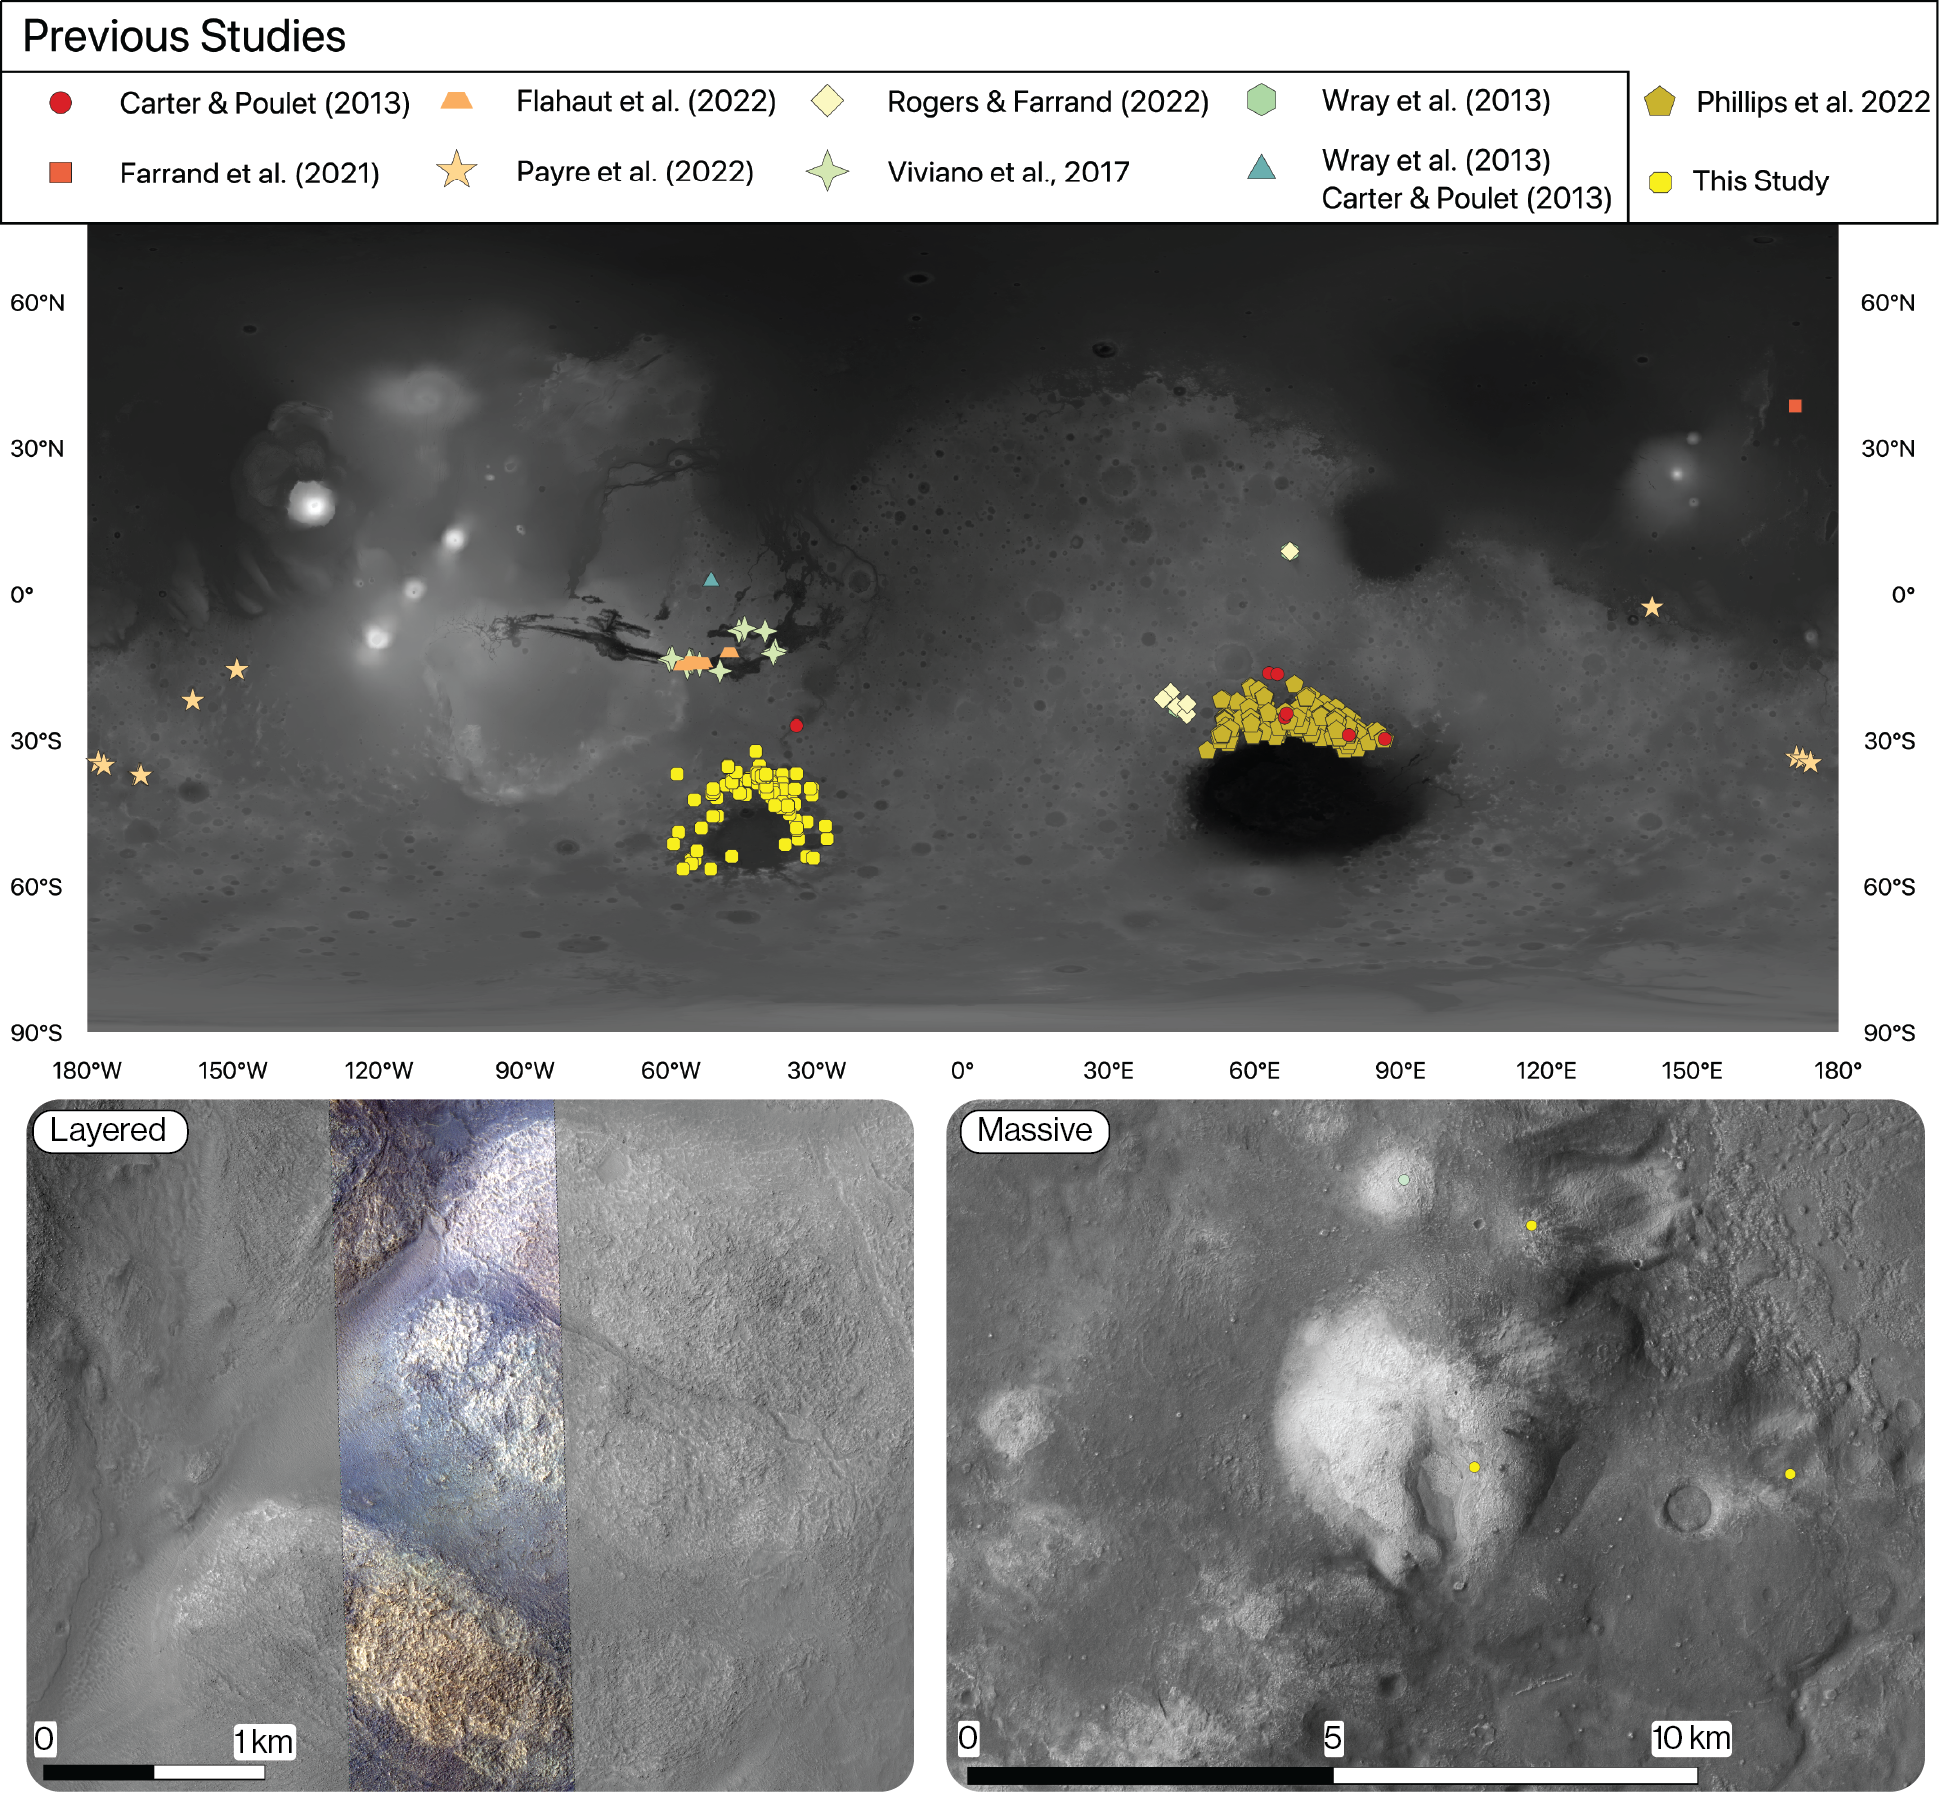
\includegraphics[width=\textwidth]
    {figures/01_Global_Context.png}
    \caption{Top panel shows the global distribution of outcrops showing a plagioclase absorption feature in visible to near-infrared reflectance spectra. Results from this study in the circum-Argyre region are shown as yellow squares. Bottom left panel shows an example of possible layering between dark and light-toned units (HiRISE scene ESP\_020799\_1385). Bottom right panel shows an example light-toned massive textured outcrops with plagioclase reflectance signatures (yellow dots, mint green = alteration $\pm$ plagioclase) from the CTX global mosaic \citep{Dickson2018}.}
    \label{fig:global_distribution}
\end{figure}

\begin{figure}
    \centering
    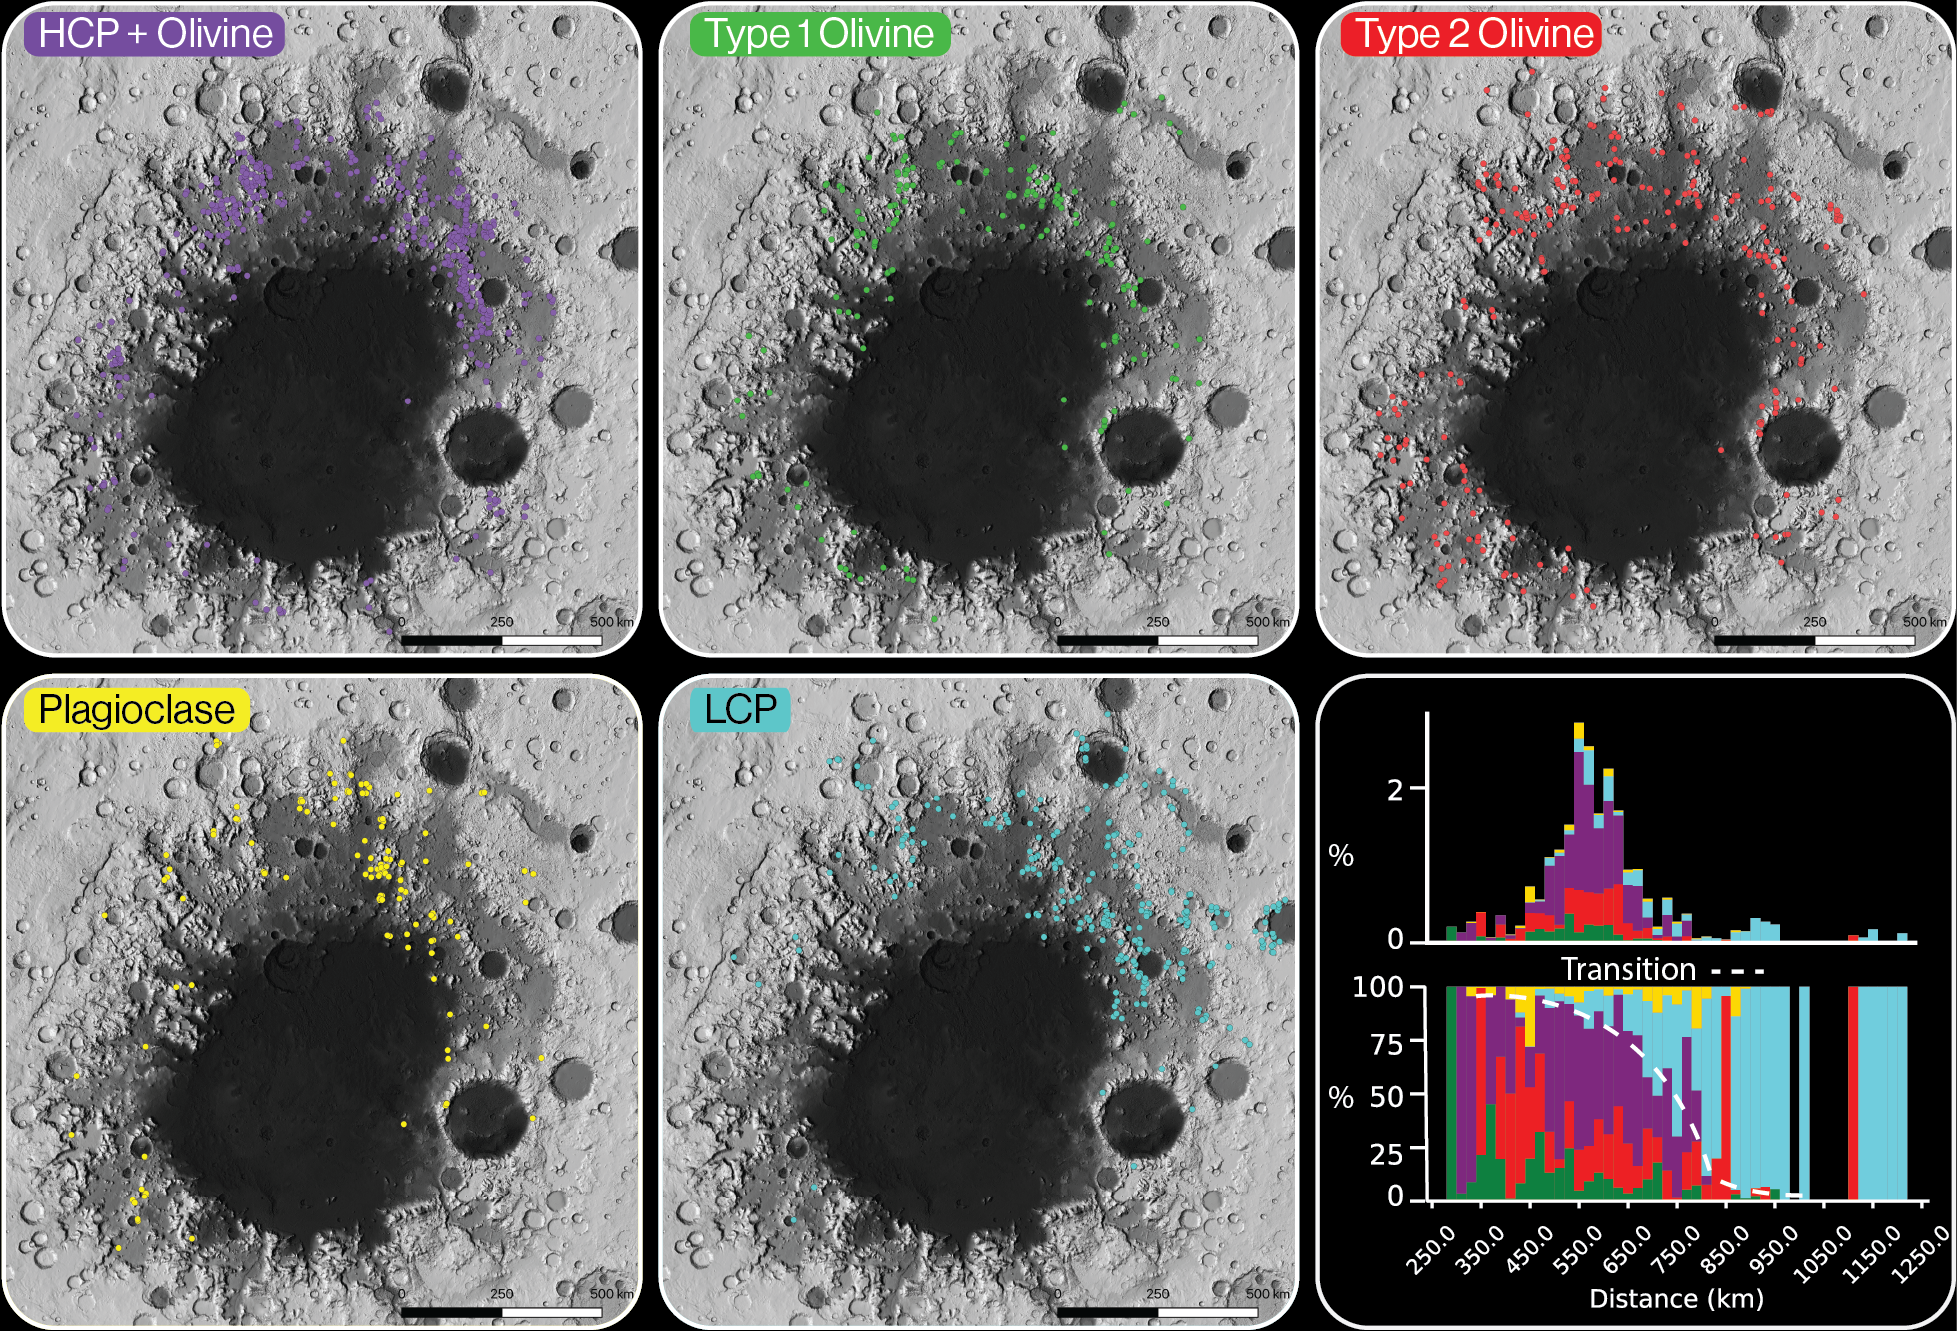
\includegraphics[width=\textwidth]
    {figures/02_Argyre_Minerals_Context_v2.png}
    \caption{Detections of high-Ca pyroxene + Olivine, type 1 and 2 olivine, plagioclase, and low-Ca pyroxene made with CRISM MRDR v4 data. The bottom right panel shows the spatial distribution of each category as a function of radial distance from the basin center binned at 20 km intervals. The top histogram is normalized to the area of geological units from \citet{Dohm2015} investigated within each ring, and the bottom histogram is normalized by the total area of detections with each ring to elucidate relative trends in the data.}
    \label{fig:detections}
\end{figure}

\begin{figure}
    \centering
    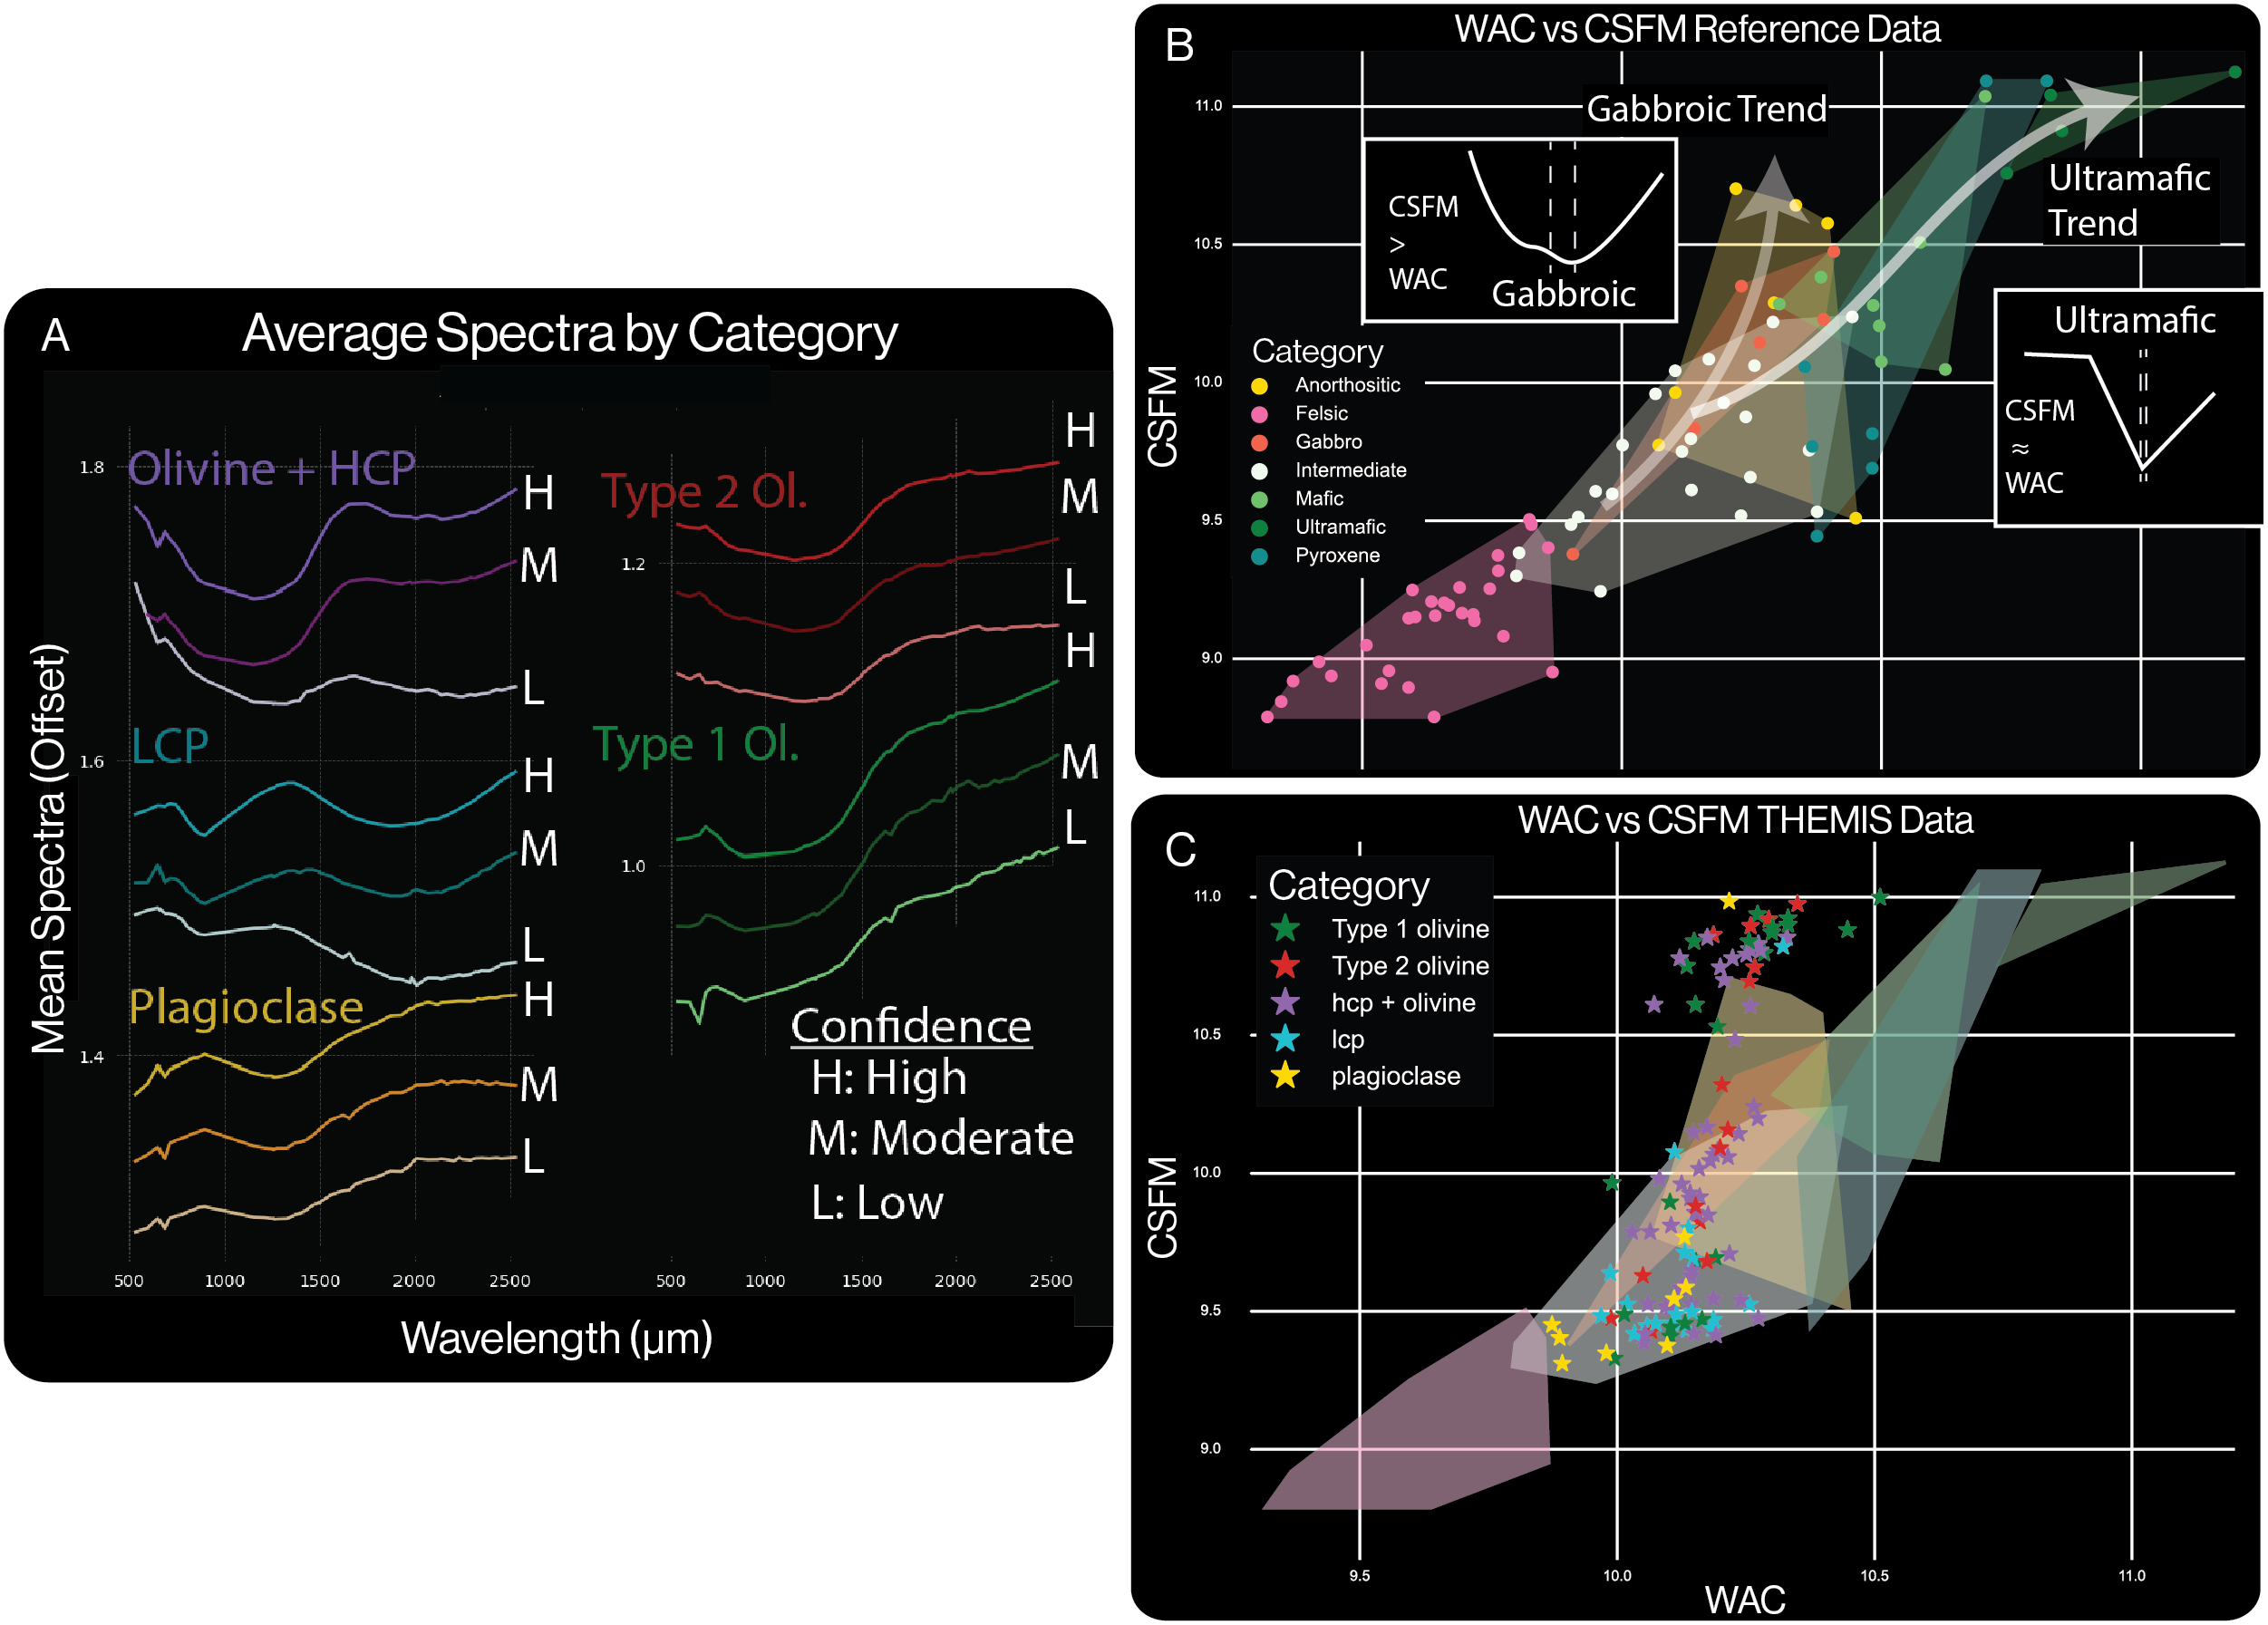
\includegraphics[width=\textwidth]
    {figures/03_spectra_figv3.png}
    \caption{Reflectance and emissivity spectral character of outcrops surrounding Argyre. A) Average CRISM spectra (ratioed I/F, offset for clarity) for each category separated by low (L), moderate (M) and high (H) confidence based on absorption strength and clarity. B) Weighted absorption center (WAC) and cubic spline fit minimum (CSFM) values calculated on THEMIS-convolved reference library data (see methods for details) of felsic, intermediate, mafic, ultramafic, gabbroic, anorthositic, and pyroxenitic rocks. Anorthositic and gabbroic rocks show a trend of higher CSFM values compared to WAC values and pyroxenitic and ultramafic rocks tend to have closer to 1:1 correspondence between CSFM and WAC values. C) WAC and CSFM values calculated on ROIs detected with CRISM (THEMIS IDs: I09614002, I09639003, I17888007, I18025006) with regions from reference library spectra for interpretation. Outcrops show the highest overlap with intermediate, gabbroic, and anorthositic compositions.}
    \label{fig:spectra}
\end{figure}

\begin{figure}
    \centering
    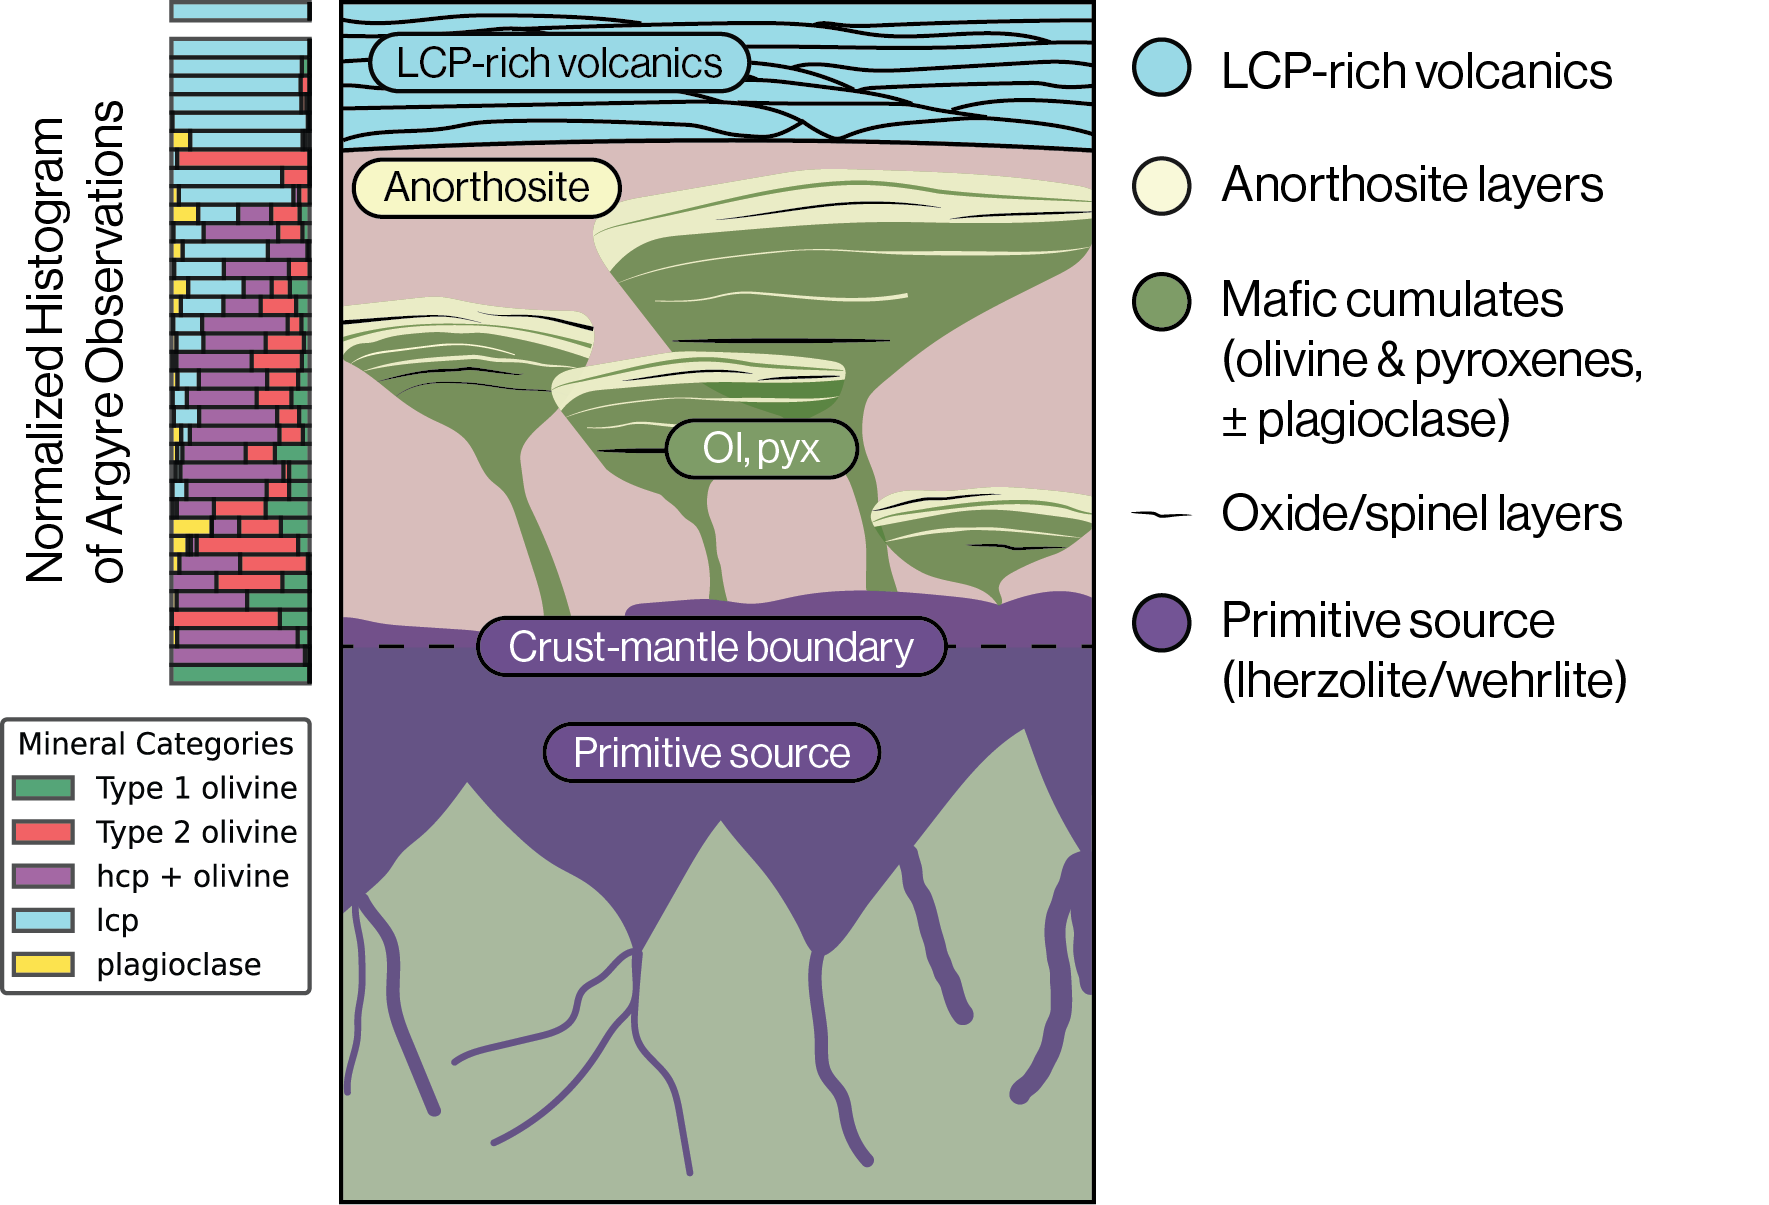
\includegraphics[width=\textwidth]
    {figures/04_crust_strat_sketch_v2.png}
    \caption{Conceptual model for the pre-Noachian crust exposed by the Argyre impact. A primitive source of possible lherzolitic or wehrlitic composition produces basaltic melt extracts that undergo fractional crystallization at lower pressures to form layered-mafic-intrusion style complexes, likely containing oxide and spinel horizons. Low-Ca pyroxene rich volcanics form a secondary upper crust.}
    \label{fig:concept_sketch}
\end{figure}

\end{document}